% !TEX root = ../../statikz2020/statikz2020.tex
\resizebox{0.75\textwidth}{!}{% 
    \tikz{

        \def\hi{0.1875};
        \def\radii{\hi}
        \def\extend{\hi}

        \coordinate (A) at (0,0);
        \coordinate (B) at (5,2.5);
        \coordinate (C) at (9.5,1.5);
        \coordinate (F) at (1.95,2.5);
        \coordinate (R) at (6.35,2.5);
        \coordinate (G) at (3.375,3.625) ;

        \gettikzxy{(A)}{\ax}{\ay}
        \gettikzxy{(B)}{\bx}{\by}
        \gettikzxy{(C)}{\cx}{\cy}
        \gettikzxy{(F)}{\fx}{\fy}
        \gettikzxy{(R)}{\rx}{\ry}
        \gettikzxy{(G)}{\gx}{\gy}

        \node[inner sep=0pt] (logo) at (\bx-.55cm,\by+1.2375cm)
        {
            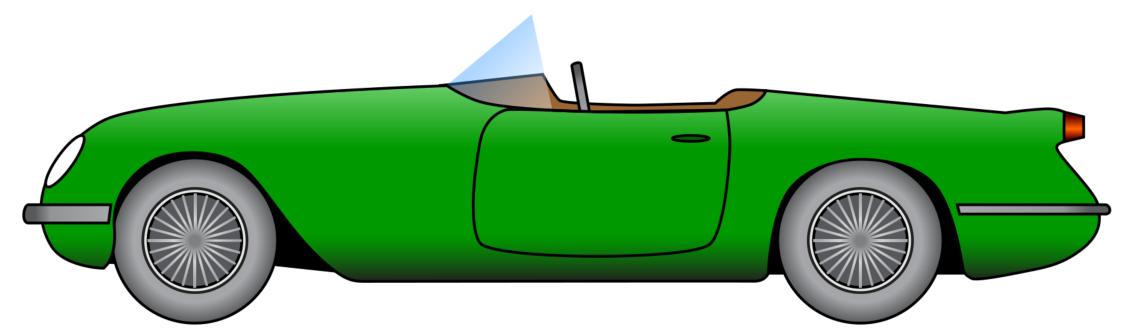
\includegraphics[scale=0.5]{../images/greenSportsCar.png}
        };

        \PinnedConnection[90]{C}{LightSteelBlue4}{black}{0.5}{0.1875}
        \PinnedConnection[-90]{A}{LightSteelBlue4}{black}{0.5}{0.1875}	

        \begin{scope}[xshift=0.1mm]
            \shade[top color=LightSteelBlue4, bottom color=LightSteelBlue1] (\ax-2.5 cm,\by+\hi cm) -- (\ax-0.5cm,\by+\hi cm) --  ++(-1, -1) -- ++(-1,0) -- (\ax-2.5 cm,\by+\hi cm);
        \end{scope}

        \shade[right color=LightSteelBlue4, left color=LightSteelBlue1] (\ax-.5 cm,\by+\hi cm) -- (\ax-0.5cm,\ay-0.75 cm) --  ++(-1, -1) -- (\ax-1.5 cm,\by-1cm +\hi cm) -- (\ax-.5 cm,\by+\hi cm);

        \begin{scope}[yshift=0.05mm]
            \shade[top color=LightSteelBlue4,bottom color=LightSteelBlue1] (\ax-0.5cm, \ay-0.75 cm) -- (\cx+\hi+0.5 cm,\ay-0.75cm) -- +(1,-1) -- (\ax-1.5 cm, \ay-1.75cm) -- cycle;
        \end{scope}

        \shade[left color=LightSteelBlue4, right color=LightSteelBlue1] (\cx+\hi+0.5 cm,\ay-0.75cm) -- (\cx+\hi+0.5 cm,\by+\hi cm) --  ++(1, -1) -- (\cx+1.5 cm,\ay-1.75cm) -- (\cx+\hi+0.5 cm,\ay-0.75cm);

        \begin{scope}[xshift=-0.1mm, yshift=-0.1mm]
            \shade[top color=LightSteelBlue4,bottom color=LightSteelBlue1] (\cx+0.5cm, \by+\hi cm) --  (\cx+2.5cm, \by+\hi cm)-- ++(0,-1) -- ++(-1,0)-- (\cx+0.5cm, \by+\hi cm);
        \end{scope}

        \draw[black, line width=0.1875mm] (\ax-2.5 cm, \by+\hi cm) -- (\ax-0.5 cm, \by+\hi cm)  -- (\ax-0.5 cm, \ay-0.75 cm) -- (\cx+\hi+0.5 cm,\ay-0.75cm) -- (\cx+0.5cm, \by+\hi cm) -- ++(2,0);



        \filldraw[fill=LightSteelBlue3, draw=black, line width=0.1875mm] (\bx,\by+\hi cm) -- (\cx+\hi cm, \by+\hi cm) -- (\cx+\hi cm, \cy)arc(0:-180:\hi) -- (\cx-\hi cm,\by-\hi cm) -- (\bx, \by-\hi cm) arc(-90:-270:\hi);

        \filldraw[fill=LightSteelBlue3, draw=black, line width=0.1875mm] (\ax-\hi cm,\ay) -- (\ax-\hi cm, \by+\hi cm) -- (\bx, \by+\hi cm)arc(90:-90:\hi) -- (\ax+\hi cm,\by-\hi cm) -- (\ax+\hi cm, \ay) arc(0:-180:\hi);

        \shadedraw[ball color=LightSteelBlue4] (A) circle (3pt);
        \shadedraw[ball color=LightSteelBlue4] (B) circle (3pt);
        \shadedraw[ball color=LightSteelBlue4] (C) circle (3pt);
        \shadedraw[ball color=black] (G) circle (3pt);

        \draw (\ax,\ay-1.125cm) -- (\ax,\ay-2.875cm);
        \draw (\bx,\by-0.75cm) -- (\bx,\ay-2.875cm);
        \draw (\cx,\cy-0.75cm) -- (\cx,\ay-2.875cm);
        \draw (\rx,\ry-0.75cm) -- (\rx,\ay-2.875cm);
        \draw (\fx,\fy-0.75cm) -- (\fx,\ay-2.875cm);
        \draw (\gx,\gy-0.25cm) -- (\gx,\ay-2.875cm);
        %
        \draw (\cx-1.5cm,\cy) -- (\cx-0.375cm, \cy);
        \draw (\ax+0.375cm,\ay) -- (\cx-0.375cm,\ay);
        \draw (\cx-1.5cm,\by) -- (\cx-0.375cm, \by);

        \draw[latex-latex] (\ax,\ay-2.55cm) -- (\fx,\ay-2.55cm);        
        \draw[latex-latex] (\fx,\ay-2.55cm) -- (\gx,\ay-2.55cm);
        \draw[latex-latex] (\gx,\ay-2.55cm) -- (\bx,\ay-2.55cm);
        \draw[latex-latex] (\bx,\ay-2.55cm) -- (\rx,\ay-2.55cm);
        \draw[latex-latex] (\rx,\ay-2.55cm) -- (\cx,\ay-2.55cm);

        \draw[latex-latex] (\bx*0.2+\cx*0.8,\by) -- (\bx*0.2+\cx*0.8,\cy);
        \draw[latex-latex] (\bx*0.2+\cx*0.8,\cy) -- (\bx*0.2+\cx*0.8,\ay);

        \node[yshift=-0.4cm] at (A) {\large $A$};
        \node[yshift=-0.4cm] at (B) {\large $B$};
        \node[yshift=-0.4cm] at (C) {\large $C$};
        \node[above left] at (G) {\large $G$};
        \node[yshift=-0.4cm] at (F) {\large $F$};
        \node[yshift=-0.4cm] at (R) {\large $R$};
    }
}
